\documentclass{beamer}

\mode<presentation>
{
  \usetheme{CambridgeUS}
  \usecolortheme{beaver}
  \usefonttheme{default}
  \setbeamertemplate{navigation symbols}{}
  \setbeamertemplate{caption}[numbered]
}

\usepackage[english]{babel}
\usepackage[utf8x]{inputenc}
\usepackage{color}
\usepackage{minted}
\usemintedstyle{native}

\title[IAP-2017]{Using Computational Resources in Optimization and Statistics}
\author{Sébastien Martin}
\institute{MIT}
\date{Tuesday 01/24/2017}

\begin{document}

\begin{frame}
  \titlepage
\end{frame}


\section{Motivation}

\begin{frame}{Heavy Computations}
  In Optimization and Statistics, we often need a lot of computational power:
  \begin{itemize}
    \item Machine Learning on large datasets
    \item Hard optimization problems, mixed integer programming
  \end{itemize}
  \pause
  Or repetitive computations:
  \begin{itemize}
    \item Parameter tuning
    \item Benchmarking
  \end{itemize}
\end{frame}

\begin{frame}{Limitations of a Personal Computer}
  Using your personal computer may seem simple, but there are serious limitations:
  \begin{itemize}
    \item<1-> Limited \alert{memory} (Big Data, large matrices...)
    \item<2-> Limited \alert{computational power}.
    \item<3-> Limited \alert{number of machines}/cores.
    \item<4-> Limited \alert{time} available. (you want to use your laptop for other things too..)
  \end{itemize}
\end{frame}

\begin{frame}{How does it work : using a remote computer}
  \begin{figure}
    
\includegraphics[width=\linewidth]{figures/iap2017-diagram1}
  \end{figure}
  An interactive remote control is the easiest way to use another computer.
  \begin{itemize}
    \item We use \alert{SSH} (see lecture 1) to control a terminal on a remote machine through our computer.
    \item We can use the \alert{console} to do almost anything on the remote computer: create files, run a program, use Julia...
    \item It is also possible to use graphical softwares like \alert{R-Studio or Matlab}.
    \item It works with any computer, including your own machines.
  \end{itemize}
\end{frame}

\begin{frame}{How does it work : using a cluster}
  \begin{figure}
    \only<1>{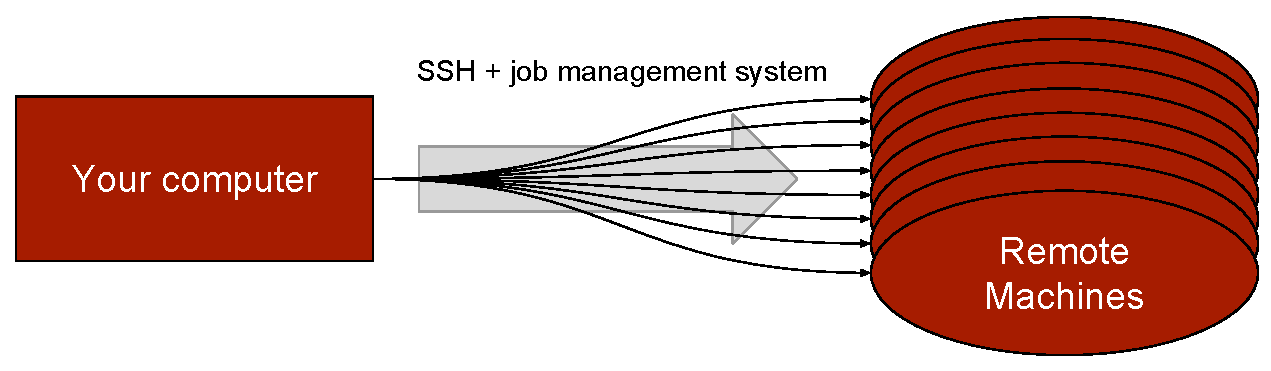
\includegraphics[width=\linewidth]{figures/iap2017-diagram2}}
    \only<2>{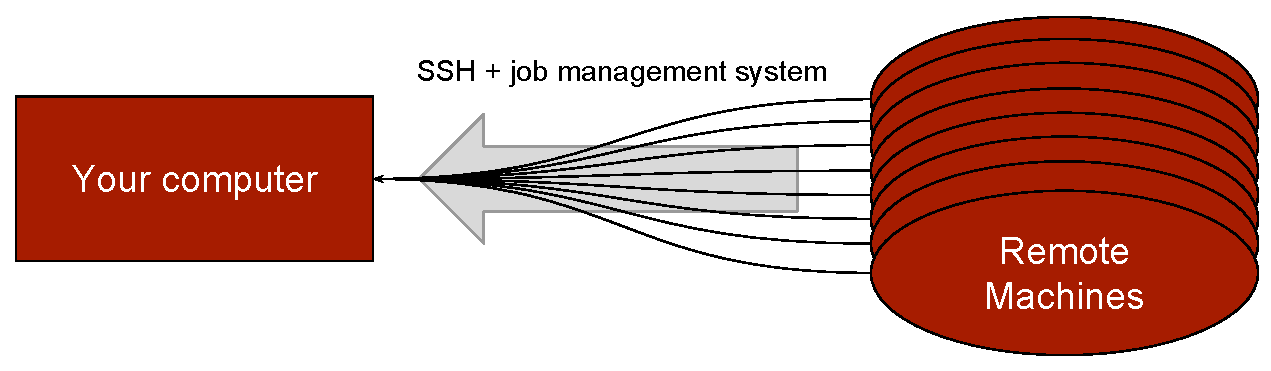
\includegraphics[width=\linewidth]{figures/iap2017-diagram3}}
  \end{figure}
  When a computing cluster is available, we can run multiple ``jobs'' thanks to a \alert{job management system}.
  \begin{itemize}
    \item Allows us to use multiple remote machines, manages demand and resources available.
    \item Different job management systems exist, I will use the example of Slurm, available to Sloan and ORC students on the cluster \alert{Engaging}.
    \item More complex to use, but far more \alert{powerful}.
  \end{itemize}
\end{frame}

\begin{frame}{Resources}
  There are several ways to have access to a remote computer or a cluster.
  \begin{itemize}
    \item Another personal computer you own.
    \item Athena at MIT.
    \item Resources of your department/lab (Engaging at Sloan).
    \item Paying options: cloud computing (Amazon AWS, Google Cloud Computing...).
  \end{itemize}
\end{frame}

\begin{frame}{Why Should I Use this}
  For research:
  \begin{itemize}
    \item Tackle bigger problems in Stats and Optimization.
    \item Parallelize your computations (parameter grid search in ML for example)!
    \item Longer computational times: run overnight or for a whole week!
    \item Bigger Datasets become manageable.
    \item Can be very simple to use with interactive sessions (RStudio...)
  \end{itemize}
  In general
  \begin{itemize}
    \item Simple to use, high reward (for example using RStudio).
    \item Useful skill in general, at the age of cloud computing.
    \item Good practice to learn how to use console (and GitHub).
  \end{itemize}
\end{frame}
\end{document}
